% myoArm Forward State Estimation -- Biological Cybernetics submission
%
% Build:
% cd paper && pdflatex main && bibtex main && pdflatex main && pdflatex main
%
% Typeset using the Springer Nature article template (sn-jnl.cls)
% with the [sn-mathphys, NameDate, iicol] options. Biological
% Cybernetics uses author-year citations; NameDate is therefore
% stated explicitly even though it is the sn-jnl default.

\documentclass[sn-mathphys,NameDate,iicol]{sn-jnl}

\usepackage{amsmath,amssymb,amsfonts}
\usepackage{graphicx}
\usepackage{booktabs}
\usepackage{multirow}
\usepackage{textcomp}
\usepackage{manyfoot}
\usepackage{xcolor}
\usepackage{url}
\usepackage{tikz}
\usetikzlibrary{positioning,arrows.meta,calc,fit,backgrounds}
\usepackage[title]{appendix}
\usepackage{hyperref}
\hypersetup{colorlinks=true,linkcolor=blue,citecolor=blue,urlcolor=blue}

\graphicspath{{../figures/}}

\raggedbottom

\begin{document}

\title[Self-Adapting a Predictive Observer's Correction Gain]{How
a Predictive State Observer Can Self-Adapt Its Sensory
Prediction-Error Correction Gain: Closed-Loop Evidence from a
Muscle-Driven Reaching Task}

\author*[1]{\fnm{Jun} \sur{Kobayashi}}\email{kobayashi.jun184@m.kyutech.ac.jp}

\affil*[1]{\orgdiv{Department of Intelligent and Control Systems,
Graduate School of Computer Science and Systems Engineering},
\orgname{Kyushu Institute of Technology}, \orgaddress{\street{680-4
Kawazu}, \city{Iizuka}, \postcode{820-8502}, \state{Fukuoka},
\country{Japan}}}

\abstract{We ask how a forward-model-based predictive state observer
should set its sensory prediction-error correction gain during
muscle-driven reaching, and whether that gain can be adapted from
agent-available signals --- innovation history and per-episode reaching
outcome --- rather than from swept oracle labels. We evaluate a
residual-MLP forward model in a 34-muscle MyoSuite arm on an
IK-reachable below-shoulder task, deployed in closed loop with a
\emph{stabilized endpoint probe controller} that uses non-negative
least-squares muscle routing and a virtual target ramp; the controller
is a stabilized probe for evaluating state-estimation effects, not a
biological motor planner. A swept fixed-gain closed-loop oracle reveals
a \emph{delay-dependent} correction structure: with no sensory delay,
intermediate correction gains are best ($K\!=\!0.25\text{--}0.50$),
whereas with $18$-step delay observation-heavy correction wins
($K\!=\!1.0$). The forward-model-only $K\!=\!0$ ablation is not the
oracle: it is systematically worse than the best fixed $K$ by
$1.9\text{--}6.1$\,cm and shows large NNLS controller residuals
caused by long-horizon autoregressive drift; we therefore report
$K\!=\!0$ as a diagnostic. Outcome-trained reliability-adaptive
observers improve the delayed regime by $1.9\text{--}2.5$\,cm over
default reliability while remaining neutral in no-delay cells, where
the oracle is already intermediate. A feature-conditioned $\beta$
adapter that maps cell-level innovation statistics to per-field gain
parameters nearly matches a per-cell trained diagnostic in $5/6$
cells, but both remain $1.4\text{--}1.8$\,cm worse than the swept
fixed-$K$ oracle at $18$-step delay. These results separate the
delay-dependent correction structure, the forward-model-only failure
mode of $K\!=\!0$, and the remaining limits of agent-available adaptive
correction.}

\keywords{Forward model, Predictive state observer, Sensory
prediction-error correction, Adaptive correction gain, Closed-loop
motor control, Muscle-driven reaching}

\maketitle

% ============================================================
\section{Introduction}
% ============================================================

State estimation in muscle-driven manipulation faces three coupled
challenges: sensorimotor delay, observation noise, and signal-%
dependent motor noise. The internal-model view of biological motor
control answers these with a \emph{forward-model-based predictive
state observer}: an internal forward model uses efference copy to
predict the next state, and the observer corrects that prediction by
a scalar weight $K\!\in\![0,1]$ on the sensory prediction error
\cite{bernstein1967,wolpert2000}. $K{=}0$ trusts the forward
prediction (efference copy); $K{=}1$ trusts the sensor; intermediate
$K$ implements a sensory-prediction-error correction. The
innovation-update form is structurally familiar from Kalman
filtering, where the gain is derived from propagated covariance
estimates \cite{kalman1960,mehra1970,anderson1979optimal}; we do
\emph{not} propagate covariances and do not claim to implement a
full Kalman filter (Sec.\,\ref{sec:method-kalman}). Instead we treat
$K$ as a scalar (or field-wise vector) that controls how strongly
sensory prediction error corrects the current state estimate, and
ask: \emph{can the agent learn to set this gain from signals it
generates online --- innovation history and per-episode task
outcome --- rather than from per-condition $K$-sweep oracle labels?}

This question is biologically motivated. The nervous system does not
have access to a swept oracle $K^{\star}$ across noise and delay
regimes; it has access to its own prediction errors and, after
moving, to whether the limb arrived where intended. We therefore
propose a \emph{two-layer reliability-adaptive observer}.
\emph{Within-trial}, a per-channel exponentially-weighted variance
of squared innovation gives a running reliability estimate
$r_f(t)$, and a logistic
$K_f(t)\!=\!\sigma(\beta_{0,f}\!+\!\beta_{1,f}\log r_f(t))$ maps it
to a field-wise correction gain on each of the five sensory fields
into which we partition the 83-dimensional state---joint position and
velocity, muscle activation, fingertip position, and reach error
(Sec.~\ref{sec:method-reliability}). \emph{Across-trial}, Simultaneous
Perturbation Stochastic Approximation (SPSA) \cite{spall1992spsa}
updates the meta-parameters $\beta\!=\!\{\beta_{0,f},\beta_{1,f}\}$
from the per-episode reaching outcome. Neither layer accesses the
optimal $K$, the true state, or a swept oracle; both use only
signals the agent generates during reaching. The resulting object
is a computational internal-model loop in the cybernetic sense:
efference-copy-based prediction is corrected by delayed sensory
prediction error, while trial-level outcome reshapes the
reliability-to-gain rule.

We instantiate this observer on a 34-muscle MyoSuite reaching arm
\cite{caggiano2022myosuite} running in the MuJoCo simulator
\cite{todorov2012mujoco} with a residual-MLP forward model trained
under $H$-step rollout supervision ($H{=}8$) and a fixed-lag
predictive state observer that handles configurable observation
delay ($d\!\in\!\{0,18\}$\,steps) and configurable per-field
Gaussian noise. To deploy the observer in closed loop without
confounding state-estimation effects with controller failure modes,
we use a \emph{stabilized endpoint probe controller}: a task-space
PD on the tip error projected to non-negative muscle activations via
non-negative least-squares (NNLS) routing, with a virtual target
ramp that prevents impulsive endpoint commands at episode onset.
The controller is a stabilized probe for evaluating state-estimation
effects, not a model of biological motor planning.

The main task analyzed in this paper is restricted to IK-reachable
targets below the neutral shoulder height ($z \!<\! 1.393$\,m),
giving a tabletop-like reaching distribution that avoids mechanically
degenerate above-shoulder IK edge solutions.

Our contributions are summarized in four claims.

\begin{itemize}
\item \textbf{C1.} \emph{The swept fixed-$K$ closed-loop oracle is
delay-dependent.} A $5$-point $K$-sweep
($K\!\in\!\{0,0.25,0.5,0.75,1\}$) across the focused
$3\,\mathrm{noise}\times\!2\,\mathrm{delay}$ grid, $n{=}200$ episodes
per cell, reveals a delay-dependent correction structure: at
delay-$0$ cells the best $K$ is intermediate
($K\!=\!0.25\text{--}0.50$, depending on noise level), while at
delay-$18$ cells the best $K$ is $K\!=\!1.0$ across all noise
levels (Fig.\,\ref{fig:F_r3_K_sweep}). The closed-loop oracle is
therefore not uniformly prediction-heavy.

\item \textbf{C2.} \emph{$K\!=\!0$ is a forward-model-only
diagnostic, not the task oracle.} $K\!=\!0$ is systematically worse
than the best fixed $K$ by $1.9\text{--}2.2$\,cm at delay-$0$ cells
and $5.2\text{--}6.1$\,cm at delay-$18$ cells (paired $95\%$
bootstrap CIs exclude zero in every cell; Fig.\,\ref{fig:F_r3_k0_diagnostic}A).
NNLS controller residuals at $K\!=\!0$ are $92\text{--}96$ across the
grid, versus $11\text{--}49$ for $K\!>\!0$
(Fig.\,\ref{fig:F_r3_k0_diagnostic}B), reflecting long-horizon
autoregressive drift that the controller cannot realize as
non-negative muscle activations. We therefore report $K\!=\!0$ as a
diagnostic ablation, not as an oracle.

\item \textbf{C3.} \emph{Outcome-trained reliability adaptation
improves the delayed regime.} Across-trial SPSA on a single global
$\beta$ improves min-tip error over the default
($\beta_{0,f}\!=\!0$, $\beta_{1,f}\!=\!0.5$) rule by
$1.85\text{--}2.46$\,cm at every delay-$18$ cell (paired $95\%$
bootstrap CIs all exclude zero), while delay-$0$ cells are
statistically neutral (Fig.\,\ref{fig:F_r3_adapt_deploy}). A
single-cell SPSA run on a representative delayed cell achieves a
$2.50$\,cm reduction over default on that cell.

\item \textbf{C4.} \emph{Feature-conditioned $\beta$ adaptation
nearly matches the per-cell-trained diagnostic for most cells, but
both remain below the swept fixed-$K$ oracle.} A
$30$-parameter linear adapter that maps z-scored log innovation
statistics to per-field $\beta$ matches a per-cell SPSA diagnostic in
$5/6$ cells (paired CIs cover zero); per-cell wins in
one zero-delay high-noise cell only, by $1.2$\,cm
(Fig.\,\ref{fig:F_r3_adapt_deploy}). However, both feature-conditioned
$\beta$ and per-cell $\beta$ remain $1.4\text{--}1.8$\,cm below the
swept fixed-$K$ oracle at every delay-$18$ cell (paired CIs all
exclude zero). Field-wise realized $K$ confirms that the adaptive
rule increases the joint-position gain from $0.72\text{--}0.92$
(default) to $0.87\text{--}0.98$ (SPSA) and suppresses the
joint-velocity gain from $0.39\text{--}0.43$ to $0.34$, but the
residual gap to the swept
oracle persists, indicating that parameterization, reliability
features, and observer dynamics jointly bound the achievable
adaptation (Fig.\,\ref{fig:F_r3_field_k}).
\end{itemize}

Together, C1--C4 separate three things that an earlier controller
diagnostic conflated: the swept-$K$ oracle structure (delay-dependent,
not uniformly $K\!=\!0$); the $K\!=\!0$ failure mode
(forward-model-only diagnostic, not a usable oracle); and the
remaining limits of agent-available adaptive correction
(observation-heavy regimes can be reached, intermediate-$K$ regimes
cannot, even with cell-conditioned $\beta$ or per-cell training).

The rest of the paper is organized as follows.
Section~\ref{sec:related} positions our work against prior literature
on adaptive correction gains and Kalman-style updates, forward models
in motor control, learned dynamics, outcome-driven adaptation, and
muscle-driven simulation.
Section~\ref{sec:method} describes the below-shoulder reaching task,
the forward model, the fixed-lag predictive state observer, the
reliability-adaptive correction-gain rule, the across-trial SPSA
loop, the stabilized endpoint probe controller, and the evaluation
pipeline.
Section~\ref{sec:results} reports the four claims with the
corresponding figures: the delay-dependent fixed-$K$ oracle
structure, the $K\!=\!0$ diagnostic, outcome-trained reliability
adaptation in delayed reaches, and the remaining gap to the swept
oracle.
Section~\ref{sec:discussion} discusses the trade-offs and the
implications of agent-available correction-gain adaptation for
biological motor control models, the role of controller-health
diagnostics in closed-loop estimator benchmarks, and the limits of
forward-model-only deployment exposed by the $K\!=\!0$ ablation.

% ============================================================
\section{Related Work}
\label{sec:related}
% ============================================================

\noindent\textbf{Adaptive correction gains and Kalman-style updates.}
The Kalman filter \cite{kalman1960} and its smoothing
counterpart~\cite{rauch1965} are the textbook framework for combining
a state-space model with noisy observations under known noise
covariances. When the covariances are unknown, the classical
\emph{adaptive Kalman filter} estimates them online from the
innovation sequence \cite{mehra1970}; the steady-state gain $K$
then drops out of the covariance estimate. We adopt the same
innovation-style update form (residual MLP for dynamics, fixed-lag
buffered correction for delays) but \emph{do not} propagate
covariances and do not compute an optimal Kalman gain; the
state-space formulation is standard textbook material
\cite{anderson1979optimal} and we treat the result as a predictive
state observer with a scalar correction gain (Sec.\,\ref{sec:method-kalman}).
The novelty of our setting is therefore not in the filter equations
but in the \emph{choice} of $K$: instead of deriving $K$ from a
noise-covariance estimate, we first measure the closed-loop fixed-$K$
oracle and then ask whether outcome-trained, agent-available
reliability adaptation can approach it without seeing oracle labels.
This closed-loop, task-outcome-driven framing is largely absent from
the adaptive-Kalman literature and is not natural inside the
covariance-propagation view.

\smallskip

\noindent\textbf{Forward and internal models in motor control.}
The view that the central nervous system maintains an internal forward
model of the limb to predict the sensory consequences of motor
commands traces back to Bernstein's degrees-of-freedom
analysis~\cite{bernstein1967} and was given an explicit computational
framing by Wolpert and Ghahramani~\cite{wolpert2000}, who identified
forward and inverse models as complementary processes underlying
sensorimotor estimation, prediction, and learning. Our residual MLP is
a coarse instantiation of the forward model in that picture; the
multi-step supervision we add is motivated by the fact that the loop
that consumes the estimate operates over hundreds of integration steps
and thus depends on long-horizon prediction quality. More biologically
grounded forward-model families --- continuous-time recurrent networks
with input-modulated time constants such as liquid time-constant
networks~\cite{hasani2021liquid} and their closed-form
variant~\cite{hasani2022cfc} --- have been proposed for sensorimotor
dynamics; in this work we keep the forward-model implementation
intentionally generic to isolate the oracle-choice question.

\smallskip

\noindent\textbf{Learned dynamics and multi-step supervision.}
Model-based reinforcement learning systems have moved from one-step
dynamics losses to multi-step rollout objectives because closed-loop
planners need predictions that survive unrolling. Dreamer
\cite{hafner2020dreamer} backpropagates through imagined trajectories
in a latent world model, and MBPO \cite{janner2019mbpo} branches
short model rollouts from real data, formalizing ``when to trust your
model''. We take the same lesson into observer design: a forward
model that is accurate enough over the controller's planning horizon
shifts where prediction-error correction is helpful and where it is
harmful.

\smallskip

\noindent\textbf{Outcome-driven adaptation and SPSA.}
Outcome-driven, gradient-free adaptation has a long history in motor
control: trial-by-trial visuomotor adaptation in humans
\cite{wolpert2000} is captured by an internal-model update rule that
uses only the observed end-of-trial error, not the underlying
optimal-gain calculation. Algorithmically, our across-trial loop
follows Spall's Simultaneous Perturbation Stochastic Approximation
(SPSA)~\cite{spall1992spsa}: a two-point gradient estimate using a
single Rademacher perturbation per iteration, with a robust
hyperparameter schedule. SPSA's appeal in this setting is that it
needs only the per-episode outcome, not the per-step state, and that
its computational cost scales with the number of meta-parameters
$\beta$ (here, $10$) rather than the dimension of the observer
state (here, $83$). Behavior cloning and DAgger
\cite{pomerleau1988alvinn, ross2011dagger} were used in an earlier
version of this work to ask whether the resulting controllers
consume state estimates; we found that with small demonstration sets,
they do not consistently expose observer differences, and we now use
only state-coupled feedback controllers in the main results, so the
observer signal flows to muscle commands.

\smallskip

\noindent\textbf{Muscle-driven simulation.}
Our task runs in MuJoCo \cite{todorov2012mujoco} via the MyoSuite
musculoskeletal benchmark \cite{caggiano2022myosuite}, which provides
a 34-muscle reaching arm and a contact-rich set of tasks suitable for
sensorimotor estimation studies. MyoSuite is increasingly used as a
testbed for reinforcement learning controllers; here, we use it instead
to ask whether a predictive state observer can adapt its
correction gain from agent-available signals alone, a question that
the RL-centric literature has not addressed.

% ============================================================
\section{Method}
\label{sec:method}
% ============================================================

\subsection{Task and Environment}
\label{sec:method-task}
We use the \texttt{myoArmReachFixed-v0} task in MyoSuite\,2.12.2, a 34-muscle
shoulder-elbow-wrist-hand system actuated by activations in $[0,1]^{34}$.
The task is to drive the index-finger tip to a fixed target in a
$12$\,s episode at $\Delta t{=}0.02$\,s (600 control steps). The flat state $x\!\in\!\mathbb{R}^{83}$ stacks joint positions
$q\!\in\!\mathbb{R}^{20}$ (\texttt{qpos}), joint velocities
$\dot q\!\in\!\mathbb{R}^{20}$ (\texttt{qvel}), muscle activations
$a\!\in\!\mathbb{R}^{34}$ (\texttt{act}), finger-tip position
$p_{\mathrm{tip}}\!\in\!\mathbb{R}^{3}$ (\texttt{tip\_pos}), target
$p_{\mathrm{tgt}}\!\in\!\mathbb{R}^{3}$ (\texttt{target\_pos}), and reach
error $e{=}p_{\mathrm{tip}}-p_{\mathrm{tgt}}\!\in\!\mathbb{R}^{3}$
(\texttt{reach\_err}). True state is
extracted from MuJoCo and used only as an oracle for evaluation; the closed
loop never accesses it (Fig.\,\ref{fig:system}).

\paragraph{Below-shoulder target set.}
Targets are sampled uniformly from the environment's task-space reach range
and accepted if a damped-Jacobian IK solver places the tip within
$1$\,cm and the target lies below the neutral shoulder height
($z \!<\! 1.393$\,m). The shoulder constraint avoids mechanically
degenerate above-shoulder IK edge solutions and yields a tabletop-like
reaching distribution; it is anatomically motivated rather than a
purely numerical post-hoc filter. We generate $n{=}200$ accepted
targets with seed offset $30{,}000$; acceptance rate is $55.9\%$
(rejections are due to the shoulder-height criterion, not IK failures).
Appendix~\ref{app:artifact}
summarizes the diagnostic rationale for this target restriction.

\begin{figure*}[t]
\centering
% Define a small color-blind-safe palette (ColorBrewer Set2 / Paired)
\definecolor{envCol}{HTML}{D9D9D9} % gray
\definecolor{obsCol}{HTML}{A6CEE3} % light blue
\definecolor{estCol}{HTML}{B2DF8A} % light green
\definecolor{fwdCol}{HTML}{FDBF6F} % light orange
\definecolor{ctlCol}{HTML}{CAB2D6} % light violet
\definecolor{evalCol}{HTML}{FB9A99} % light red (dashed eval box)
\definecolor{actCol}{HTML}{6A3D9A} % deep violet (action arrow)
\definecolor{lblBg}{HTML}{FFFFFF} % label background
\begin{tikzpicture}[
 >={Stealth[length=2.2mm,inset=0.8mm]},
 box/.style={draw=black!75, rounded corners=2.5pt, minimum height=11mm,
 align=center, font=\footnotesize, inner sep=3pt,
 line width=0.5pt},
 env/.style={box, fill=envCol, minimum width=21mm},
 obs/.style={box, fill=obsCol, minimum width=24mm},
 est/.style={box, fill=estCol, minimum width=33mm, minimum height=15mm},
 fwd/.style={box, fill=fwdCol, minimum width=29mm, font=\scriptsize,
 minimum height=10mm},
 ctl/.style={box, fill=ctlCol, minimum width=22mm},
 eval/.style={box, dashed, draw=evalCol!80!black, fill=evalCol!30,
 minimum width=29mm, font=\scriptsize\itshape},
 lbl/.style={font=\scriptsize, fill=lblBg, inner sep=1pt},
 arrlbl/.style={lbl, midway},
 flowarr/.style={->, line width=0.55pt},
 actarr/.style={->, line width=0.8pt, color=actCol},
 evalarr/.style={->, dashed, color=evalCol!70!black, line width=0.5pt},
 node distance=6mm and 12mm,
]
% --- Main horizontal flow ---
\node[env] (env) {MuJoCo /\\MyoSuite};
\node[obs, right=of env] (obs) {Obs.\ wrappers\\noise $+$ delay};
\node[est, right=of obs] (est) {State observer\\
 $\hat x_t {=} x_{\mathrm{pred}} {+} K\!\cdot\!(y_t{-}x_{\mathrm{pred}})$};
\node[ctl, right=of est] (ctl) {Controller\\stabilized probe};

% --- Forward model below estimator ---
\node[fwd, below=11mm of est] (fwd)
 {forward model $f_\theta$\\(residual MLP)};

% --- Evaluation-only oracle (kept off the control-action return path) ---
\node[eval, above=8mm of env] (eval)
 {true state $x_t$\\(oracle, eval only)};

% --- Flow arrows ---
\draw[flowarr] (env) -- node[arrlbl,above]{$x_t$} (obs);
\draw[flowarr] (obs) -- node[arrlbl,above]{$y_t$} (est);
\draw[flowarr] (est) -- node[arrlbl,above]{$\hat x_t$} (ctl);

% --- Forward-model bidirectional connection ---
% Up arrow on the left -- forward model returns x_pred.
\draw[flowarr] ($(fwd.north west) + (8mm,0)$)
 -- node[lbl,pos=0.45]{$x_{\mathrm{pred}}$}
 ($(est.south west) + (8mm,0)$);
% Down arrow on the right -- estimator feeds (x_hat,u) at last step.
\draw[flowarr] ($(est.south east) + (-8mm,0)$)
 -- node[lbl,pos=0.55]{$\hat x_{t{-}1},\, u_{t{-}1}$}
 ($(fwd.north east) + (-8mm,0)$);

% --- Closed-loop action arrow (controller -> env, routed underneath) ---
\draw[actarr] (ctl.south) -- ++(0,-25mm) coordinate (botctl)
 -| node[arrlbl,below=1mm,pos=0.45]
 {$u_t \in [0,1]^{34}$ \textit{(muscle exc.)}}
 (env.south east);

% --- Eval arrow (oracle path; visually subdued) ---
\draw[evalarr] (env.north) -- node[lbl,midway,fill=white]{oracle}
 (eval.south);

% --- Background dashed box for closed loop ---
\begin{scope}[on background layer]
\node[draw=black!35, dashed, rounded corners,
 fit=(env)(obs)(est)(ctl)(fwd),
 inner sep=4mm,
 label={[font=\scriptsize\itshape,anchor=north east]north east:closed
 loop (no true state)}] {};
\end{scope}
\end{tikzpicture}
\caption[Closed-loop pipeline.]%
{\textbf{Closed-loop pipeline.} Each control step, the environment's true
state $x_t$ is filtered through observation wrappers that add
per-field Gaussian noise and a fixed delay, producing $y_t$. The
predictive state observer combines $y_t$ with a one-step
prediction $x_{\mathrm{pred}}$ produced by the residual-MLP forward
model $f_\theta(\hat x_{t-1}, u_{t-1})$ via a scalar correction gain
$K\!\in\![0,1]$ on the sensory prediction error $y_t - x_{\mathrm{pred}}$,
as in Eq.~(\ref{eq:kalman_update}). The controller consumes only the
observer output $\hat x_t$ and emits the next muscle excitation
$u_t\!\in\![0,1]^{34}$. The true state $x_t$ is exposed only to the
offline evaluator (dashed red box); the closed loop never accesses
it.}
\label{fig:system}
\end{figure*}

\subsection{Forward Model}
A residual MLP $f_\theta(x_t, u_t)$ predicts the state delta
$\Delta x_t {=} x_{t+1}-x_t$ rather than $x_{t+1}$ directly. At
$\Delta t{=}0.02$\,s the state changes slowly, so $x_{t+1}\!\approx\!x_t$
component-wise; predicting $\Delta x$ frees the model from re-learning
the identity map and concentrates capacity on the small per-step
dynamics that the filter and controller actually consume. The
parameterization is standard in model-based RL world
models~\cite{hafner2020dreamer,janner2019mbpo}. The input is the flat
83-dimensional state and the 34-dimensional excitation; the architecture is two hidden
layers of 256 units with ReLU and LayerNorm; training uses
Adam~\cite{kingma2015adam}.
In the single-step baseline, $f_\theta$ is trained on the standard
one-step MSE loss
\begin{equation}
\mathcal{L}_1(\theta) = \mathbb{E}_{(x_t,u_t,x_{t+1})}\big[\|f_\theta(x_t,u_t)
- \Delta x_t\|^2\big].
\label{eq:L_one_step}
\end{equation}

\noindent\textbf{Multi-step rollout supervision.} The multi-step
variant trains $f_\theta$ with an $H$-step rollout loss instead of
the one-step MSE, where $H$ denotes the training rollout horizon.
For each contiguous trajectory chunk
$(x_t,u_t,\dots,x_{t+H})$ inside a single source episode, the model
is unrolled free-running:
$\hat x_{t+k} = \hat x_{t+k-1} + f_\theta(\hat x_{t+k-1}, u_{t+k-1})$,
$\hat x_t = x_t$, and the loss averages MSE across the $H$
prediction steps:
\begin{equation}
\mathcal{L}_H(\theta) = \mathbb{E}\Big[\tfrac{1}{H}\sum_{k=1}^H\|\hat x_{t+k}
- x_{t+k}\|^2\Big].
\label{eq:L_H_step}
\end{equation}
Multi-step rollout supervision has been used to stabilize long-horizon
predictions in latent-imagination world models~\cite{hafner2020dreamer}
and in model-based policy optimization~\cite{janner2019mbpo}, where the
relevant horizon is the planner's rollout depth rather than the
observer's delay; we re-use the technique here to make $f_\theta$
robust across the observer's buffer rollout.

\noindent We train the same architecture with $H\!\in\!\{1,4,8\}$ on the
expanded reachable-target dataset
(77\,k transitions across 150 episodes; see
Appendix~\ref{app:fwd-rollout}).

\subsection{Fixed-Lag Predictive State Observer}
\label{sec:method-kalman}
The observer uses an innovation-update form structurally familiar
from Kalman filtering, but does not propagate covariances and does
not compute an optimal Kalman gain. The gain $K\!\in\![0,1]$ is a
\emph{sensory prediction-error correction gain}, not a covariance-%
derived Kalman gain.

The observation pipeline produces $y_t = x_{t-d} + \eta_t$, where the
observation shares the same schema as the $83$-dimensional state vector,
$d\!\in\!\mathbb{Z}_{\geq 0}$ is a fixed delay in control steps, and
$\eta_t$ is per-field i.i.d.\ Gaussian noise with diagonal covariance
$\mathrm{diag}(\sigma^2)$. The estimator maintains
a length-$(d{+}1)$ ring buffer of past one-step estimates
$(\hat x_{t-d}, \dots, \hat x_{t-1})$ together with the corresponding
applied actions $(u_{t-d}, \dots, u_{t-1})$. At each step, the
observer first runs the forward model on every buffered estimate to
obtain a prediction at the present time,
\begin{equation}
\tilde x_t = \hat x_{t-1} + f_\theta(\hat x_{t-1}, u_{t-1}),
\end{equation}
then forms an innovation against the \emph{delayed} buffer entry and
applies an element-wise gain $K\!\in\![0,1]^{83}$:
\begin{equation}
\hat x_{t-d}
\leftarrow
\hat x_{t-d} + K \odot \bigl(y_t - \hat x_{t-d}\bigr),
\label{eq:kalman_update}
\end{equation}
and finally re-rolls the corrected past estimate forward through the
buffered actions to obtain the present-time estimate $\hat x_t$.
Eq.~(\ref{eq:kalman_update}) collapses to the standard one-step
innovation update when $d{=}0$. Throughout the paper $K$ is a scalar
broadcast across the 83 state coordinates so the correction gain reduces to a
single trust knob between forward prediction ($K{=}0$) and
observation ($K{=}1$). This fixed-lag construction follows the
buffered Rauch--Tung--Striebel form~\cite{rauch1965,anderson1979optimal}
specialized to a scalar gain.

\paragraph{Noise and delay grids.}
The main closed-loop experiments use a focused grid with delays
$d\!\in\!\{0,18\}$ and three observation-noise presets. We denote
the categorical noise level by
$\nu\!\in\!\{\mathrm{none},\mathrm{high},\mathrm{xhigh}\}$. The label
\emph{none} sets all observation-noise standard deviations to zero;
\emph{high} uses $\sigma_{\mathrm{qpos}}=\sigma_{\mathrm{qvel}}=0.02$
and $\sigma_{\mathrm{tip}}=\sigma_{\mathrm{reach}}=0.01$; \emph{xhigh}
uses $\sigma_{\mathrm{qpos}}=\sigma_{\mathrm{qvel}}=0.08$ and
$\sigma_{\mathrm{tip}}=\sigma_{\mathrm{reach}}=0.04$. These labels are
used only as compact table and figure notation for the corresponding
per-field Gaussian noise settings (the sensory fields are defined in
Sec.~\ref{sec:method-reliability}).

\subsection{Reliability-Adaptive Correction Gain (Within-Trial)}
\label{sec:method-reliability}
The observer above uses a fixed scalar $K$ broadcast across all 83
fields. We propose instead an \emph{agent-available, field-wise
reliability-adaptive} rule that sets $K_f(t)$ online from each
sensory channel's own innovation history. No oracle on the optimal
gain, no true state, and no swept-condition labels enter the rule;
only the per-step innovation $e_t \!=\! y_t \!-\! \hat x_{t-d}$ does.

We partition the 83-dimensional state into five adaptive \emph{sensory
fields}---20-D \texttt{qpos}, 20-D \texttt{qvel}, 34-D \texttt{act},
3-D \texttt{tip\_pos}, and 3-D \texttt{reach\_err}---and a sixth,
3-D fixed-gain target channel, \texttt{target\_pos}. The
partition is an engineering grouping driven by the MyoSuite state
schema, but it admits a coarse biological reading: \texttt{qpos} and
\texttt{qvel} are proprioceptive-like, \texttt{act} is efferent and
muscle-command-like, and \texttt{tip\_pos} and \texttt{reach\_err} are
visual and task-space-like. The
3-D target-position channel is held at a fixed gain because the
target is known and does not have a meaningful prediction error.
For each field $f\!\in\!\mathcal{F}\!=\!\{\mathrm{qpos},
\mathrm{qvel}, \mathrm{act}, \mathrm{tip\_pos},
\mathrm{reach\_err}\}$ the observer maintains an exponentially-%
weighted (EMA) estimate of the per-field squared-innovation mean,
\begin{equation}
v_f(t) = (1-\alpha)\,v_f(t-1) + \alpha\;
 \frac{1}{|\mathcal{I}_f|}\sum_{i \in \mathcal{I}_f} e_{t,i}^{2},
\label{eq:ema_innovation_var}
\end{equation}
where $\mathcal{I}_f$ are the field's coordinate indices in the
83-dimensional state vector and $\alpha\!=\!0.05$ unless otherwise noted.
The agent's running estimate of \emph{sensory reliability} for
field $f$ is the inverse of this variance,
\begin{equation}
r_f(t) = \frac{1}{\varepsilon + v_f(t)},
\label{eq:reliability}
\end{equation}
with $\varepsilon\!=\!10^{-6}$. We then map reliability to a
per-field correction gain through a two-parameter logistic,
\begin{equation}
K_f(t) = \sigma\bigl(\beta_{0,f} + \beta_{1,f}\,\log r_f(t)\bigr),
\quad \sigma(z)\!=\!\frac{1}{1+e^{-z}},
\label{eq:Kf_logistic}
\end{equation}
and form the 83-dimensional gain vector $K(t)\!\in\![0,1]^{83}$ by
broadcasting $K_f(t)$ over its field's coordinates. The
innovation update in Eq.~(\ref{eq:kalman_update}) is then applied
elementwise with $K(t)$ in place of the scalar $K$.

Eq.~(\ref{eq:Kf_logistic}) is intentionally simple. The slope
$\beta_{1,f}$ controls how sharply the gain reacts to changes in
log-reliability, and the intercept $\beta_{0,f}$ controls the
operating point at $r_f(t)\!=\!1$ (i.e., $K_f\!=\!\sigma(\beta_{0,f})$).
With $\beta_{0,f}\!=\!0$, $\beta_{1,f}\!=\!0.5$, and $v_f(0)\!=\!1$,
the rule produces $K_f(t)\!\approx\!0.5$ on the first step and
adapts upward when innovation shrinks (the sensor is informative) or
downward when innovation grows (the sensor is noisy). Per-field
$\beta\!=\!\{\beta_{0,f}, \beta_{1,f}\}$ lets the rule learn that
different fields have different reliability--correction trade-offs
under the same physical noise level.

\subsection{Across-Trial Outcome Adaptation (SPSA)}
\label{sec:method-spsa}
The meta-parameters $\beta\!=\!\{(\beta_{0,f}, \beta_{1,f}):
f\!\in\!\mathcal{F}\}\!\in\!\mathbb{R}^{10}$ themselves can be
adapted across trials from \emph{outcome} signals the agent has at
the end of each episode. We define the per-episode outcome as the
minimum tip-to-target distance,
\begin{equation}
\mathrm{minTip}(\beta;\,\nu,d) \;=\;
 \min_{t\in[0,T]}\,\|p_{\mathrm{tip}}(t) - p_{\mathrm{tgt}}\|,
\label{eq:outcome}
\end{equation}
computed from the simulated trajectory after each episode. We use
$\mathrm{minTip}$ as an \emph{operational scalar outcome} for
across-trial optimization, not as a biological claim that an agent
directly observes the trajectory minimum. The across-trial loop minimizes
$\mathbb{E}[\mathrm{minTip}(\beta)]$ where the expectation is over
target draws (and, in the multi-cell variant, over uniformly drawn
$(\nu, d)$ cells from the focused grid).

Because the closed-loop $\mathrm{minTip}$ is not differentiable in
$\beta$ (it passes through environment steps, EMA state, and a non-smooth
$\min$), we use Simultaneous Perturbation Stochastic Approximation
(SPSA)~\cite{spall1992spsa}: at iteration $n$, draw a Rademacher
vector $\Delta_n\!\in\!\{\pm 1\}^{10}$, evaluate the outcome at
$\beta_n \pm c_n \Delta_n$ averaged over $S$ paired episodes
(samples per side), form the central-difference gradient estimate
\begin{equation}
\begin{aligned}
\hat g_n
 &= \frac{\delta_n}{2 c_n}\,\Delta_n^{-1},\\
\delta_n
 &= \mathrm{minTip}(\beta_n + c_n\Delta_n)
  - \mathrm{minTip}(\beta_n - c_n\Delta_n),
\end{aligned}
\label{eq:spsa_grad}
\end{equation}
and update $\beta_{n+1} \!=\! \beta_n - a_n \hat g_n$. The Spall
schedules are $a_n \!=\! a / (n{+}1{+}A)^{\alpha_s}$ and
$c_n \!=\! c / (n{+}1)^{\gamma_s}$ with $a{=}2.0$, $c{=}0.3$,
$\alpha_s{=}0.602$, $\gamma_s{=}0.101$, and $A{=}5$. Two SPSA
variants are reported: \emph{single-cell} ($S{=}12$, $100$
iterations, no-noise, $d{=}18$) and \emph{full-grid}
($S{=}12$, $100$ iterations, uniformly drawn $(\nu,d)$ from the
$6$-cell grid per iteration).

\subsection{Feature-Conditioned $\beta$ Adapter}
\label{sec:method-fc}
\label{sec:method-feature-cond}

\S\ref{sec:method-spsa} optimizes one global
$\beta\!\in\!\mathbb{R}^{10}$ and deploys that same reliability-to-gain
map in every noise/delay cell. The feature-conditioned adapter asks
whether $\beta$ can be adjusted from information available inside the
cell itself: the magnitude and variance of each field's recent
innovation. We start from a fixed base parameter
$\beta^{\mathrm{base}}$ and add a small independent linear correction
for each sensory field.

\paragraph{Architecture.}
For each sensory field $f \!\in\! \mathcal{F}$, the adapter outputs a
correction $(\Delta\beta_{0,f}, \Delta\beta_{1,f})$ from two
per-field features:
\begin{equation}
\begin{aligned}
\Delta\beta_{0,f}
 &= w^{(0)}_{\mathrm{mean},f} \, z_{\mathrm{mean},f}
 + w^{(0)}_{\mathrm{var},f} \, z_{\mathrm{var},f}
 + b^{(0)}_f, \\
\Delta\beta_{1,f}
 &= w^{(1)}_{\mathrm{mean},f} \, z_{\mathrm{mean},f}
 + w^{(1)}_{\mathrm{var},f} \, z_{\mathrm{var},f}
 + b^{(1)}_f,
\end{aligned}
\label{eq:feature_cond_adapter}
\end{equation}
giving five fields $\times$ two outputs $\times$ three weights
$=30$ parameters total. The effective per-field $\beta$ used by the
within-trial layer is
\begin{equation}
\beta_{0,f}^{\mathrm{eff}} = \beta_{0,f}^{\mathrm{base}}
 + \Delta\beta_{0,f},
\qquad
\beta_{1,f}^{\mathrm{eff}} = \beta_{1,f}^{\mathrm{base}}
 + \Delta\beta_{1,f},
\label{eq:feature_cond_beta}
\end{equation}
fixed for the duration of one episode. Setting all 30 adapter
weights to zero recovers $\beta^{\mathrm{base}}$ exactly, so the
adapter is an additive correction. Throughout the main results we
take $\beta^{\mathrm{base}}$ to be the global SPSA $\beta$ trained
on the focused grid (Sec.\,\ref{sec:method-spsa}).

\paragraph{Input features and normalization.}
The two per-field features $z_{\mathrm{mean},f}$ and
$z_{\mathrm{var},f}$ are agent-available innovation statistics:
mean absolute innovation and mean squared innovation over the
second half of a brief default-reliability warm-up run on the cell.
Each statistic is then log-transformed and z-scored \emph{across the
focused-grid cells} using normalization constants estimated once
from the warm-up rollouts and then frozen:
\begin{equation}
z_{\bullet,f}
 = \frac{\log(1 + s_{\bullet,f}) - \mu_{\bullet,f}^{\mathrm{norm}}}
 {\sigma_{\bullet,f}^{\mathrm{norm}}},
\end{equation}
where $s_{\bullet,f}$ is the raw statistic and
$(\mu^{\mathrm{norm}}, \sigma^{\mathrm{norm}})$ are calibration
constants. This calibration is analogous to sensory scale
calibration in a biological agent: it adjusts the units of
innovation features into a common scale, but does not encode the
optimal correction gain or any oracle label.

\paragraph{Training.}
The 30 adapter weights are trained by SPSA on the same per-episode
$\min$-tip outcome used in Sec.\,\ref{sec:method-spsa}, with
$200$ iterations, $S\!=\!12$ paired episodes per iteration (two
samples per cell, six cells), perturbation amplitude $c\!=\!0.3$
and learning rate $a\!=\!0.5$, both annealed by the Spall schedule.
The cell features computed in the calibration step are reused at
each iteration without modification --- the adapter learns a single
context-to-$\beta$ map, not a per-cell $\beta$.

\subsection{Controllers}
\label{sec:method-controller}
All main closed-loop results use a single \emph{stabilized endpoint probe
controller}. We retain it only because we need a closed-loop probe
that does not by itself fail in muscle space; it is not a model of
biological motor planning and not a candidate optimal-control policy.

\paragraph{Stabilized endpoint probe.}
A task-level PD law on the estimated tip-to-target error is projected
into the non-negative muscle-activation cone via non-negative least
squares against the actuator moment-arm matrix
$M\!\in\!\mathbb{R}^{34\times 20}$, and the controller's effective
target is ramped from the initial tip position $p_{\mathrm{tip}}^{(0)}$
to the episode target $p^{\star}$ over
$T_{\mathrm{ramp}}{=}300$ steps to avoid impulsive commands at episode
onset. At control step $t$, with estimated tip position
$\hat p_{\mathrm{tip},t}$ and estimated joint velocity $\hat{\dot q}_t$,
\begin{align}
s_t &= \min\!\bigl(t / T_{\mathrm{ramp}},\,1\bigr),
\label{eq:ramp_fraction}\\
p^{\diamond}_t &= p_{\mathrm{tip}}^{(0)} + s_t\,\bigl(p^{\star} - p_{\mathrm{tip}}^{(0)}\bigr),
\label{eq:virtual_target}\\
u_{\mathrm{tip},t} &= K_{p}\bigl(p^{\diamond}_t - \hat p_{\mathrm{tip},t}\bigr)
 - K_{d}\,J\,\hat{\dot q}_t, \\
u_{\mathrm{joint},t} &= J^{\top}\,u_{\mathrm{tip},t},
\label{eq:stabilized_pd}\\
a_t &= \mathrm{argmin}_{a\geq 0}\;\bigl\lVert M^{\top}a - u_{\mathrm{joint},t}\bigr\rVert_{2}, \label{eq:nnls}\\
u_{\mathrm{muscle},t} &= \mathrm{clip}\!\bigl(\alpha\,a_t,\,0,\,1\bigr).
\label{eq:nnls_clip}
\end{align}
Here $s_t$ is the ramp fraction, $p^{\diamond}_t$ is the virtual target,
$u_{\mathrm{tip},t}$ and $u_{\mathrm{joint},t}$ are task-space and
joint-space demand vectors, $a_t$ is the non-negative NNLS routing
variable, and $u_{\mathrm{muscle},t}$ is the final muscle command. We
use $K_{p}{=}30$, $K_{d}{=}3$, $\alpha{=}5$, with $J$ the tip-site
positional Jacobian captured at the environment's neutral pose. NNLS is the
SciPy implementation of the standard active-set NNLS algorithm.

The NNLS routing in Eq.~(\ref{eq:nnls}) is used because it (i)
respects the non-negative muscle constraint without ReLU-induced
symmetry-breaking between antagonist pairs and (ii) returns a residual
norm $\lVert M^{\top}a - u_{\mathrm{joint}}\rVert_{2}$ that we log as
a per-step controller-health diagnostic. The virtual target ramp
in Eqs.~(\ref{eq:ramp_fraction})--(\ref{eq:virtual_target}) is a
transparent demand-shaping device,
not a minimum-jerk planner; we deliberately do not couple it to an
optimal-control objective.

We refer to this controller as a \emph{stabilized probe controller}
throughout. Appendix~\ref{app:artifact} summarizes the controller
diagnostic that motivated this stabilized design.

\subsection{Evaluation Pipeline}
\emph{Open-loop} evaluation replays a recorded episode and applies
observation wrappers to synthesize $y_t$ for an arbitrary $(\nu, d)$
combination; the estimator is then run on the synthesized stream and
per-field state error is aggregated. \emph{Closed-loop} evaluation drives
the actual environment: $u_t$ comes from the controller, which sees the estimator
output (never the true state). The main closed-loop fixed-$K$ sweep and
adaptive deployments use $200$ episodes per noise/delay cell with
paired episode seeds across estimators. Smaller 10-episode sweeps are
used only for historical diagnostics in Appendix~\ref{app:artifact}.
The open-loop diagnostic grid uses 3 controllers $\times$ 6 noise
levels $\times$ 4 delays; the main closed-loop grid uses the focused
3 noise levels $\times$ 2 delays defined above.

% ============================================================
\section{Results}
\label{sec:results}
% ============================================================

\subsection{Forward-model selection and h=600 long-horizon diagnostic}
\label{sec:results-forward-model}

The main forward model is a residual MLP trained with $H{=}8$ rollout
supervision on the $77{,}292$-transition reachable-target dataset
(Appendix~\ref{app:fwd-rollout}); it attains an
$h{=}50$ tip prediction error of $0.034$\,m
(full rollout metrics in Table~\ref{tab:fwd_rollout}),
which meets the open-loop validation threshold, and
is the model used in all closed-loop results below.

Because the closed-loop episode horizon is $600$ control steps, we
additionally run a zero-action $h{=}600$ autoregressive stability
diagnostic on the four forward-model variants
($H{=}1$, $H{=}4$, $H{=}8$ main, undertrained $H{=}8$;
Appendix~\ref{app:fwd-rollout}). The two $H{=}8$ variants keep
$|q|_{\max}\!\leq\!5$\,rad and
$|\dot q|_{\max}\!\leq\!10$\,rad/s under zero action; for the main
$H{=}8$ model, tip drift of $1.03$\,m is at the anatomical-workspace
boundary. The
state-vector $p_{\mathrm{tgt}}$ field drifts by $0.54$\,m even though
the environment target is invariant, a known structural limitation of
including the target field in the predicted state, which we leave as
future work.
We retain target drift as a diagnostic field, but do not include it
in the formal open-loop validation threshold
(Appendix~\ref{app:fwd-rollout}).

\subsection{Fixed-$K$ sweeps reveal delay-dependent correction structure (C1)}
\label{sec:results-c1}

We run a $5$-point closed-loop $K$-sweep
($K\!\in\!\{0,0.25,0.5,0.75,1\}$) under the stabilized endpoint
probe on the focused $3\,\mathrm{noise}\times\!2\,\mathrm{delay}$
grid, $n{=}200$ episodes per cell, with the below-shoulder
target set (Sec.\,\ref{sec:method-task}). Each estimator is a fixed-gain predictive
state observer over the $H{=}8$ forward model.

Figure~\ref{fig:F_r3_K_sweep} plots the within-cell penalty as a
function of $K$, defined as excess $\min$-tip error relative to the
best fixed $K$ in the same noise/delay cell. This normalization is
only for visualization; the absolute cell means are reported in
Table~\ref{tab:r3_bestK}. The correction structure is
delay-dependent. At delay-$0$ cells, the best fixed $K$ is
intermediate: $K\!=\!0.50$ for $\nu{=}\mathrm{none}$,
$K\!=\!0.25$ for $\nu{=}\mathrm{high}$ and
$\nu{=}\mathrm{xhigh}$. Increasing observation noise pushes the
no-delay optimum from $K\!=\!0.50$ to $K\!=\!0.25$, i.e., the
estimator favors its forward-model prediction more strongly when
the channel is noisier --- the qualitative direction expected from
reliability-weighted prediction-error correction. At delay-$18$ cells, the best fixed
$K$ collapses to $K\!=\!1.0$ across all three noise levels; the
stale forward-model prediction (delayed by the same $18$ steps as
the observation) is no longer a useful current-state anchor, and
observation-heavy correction wins despite the noise.

\begin{figure}[t]
\centering
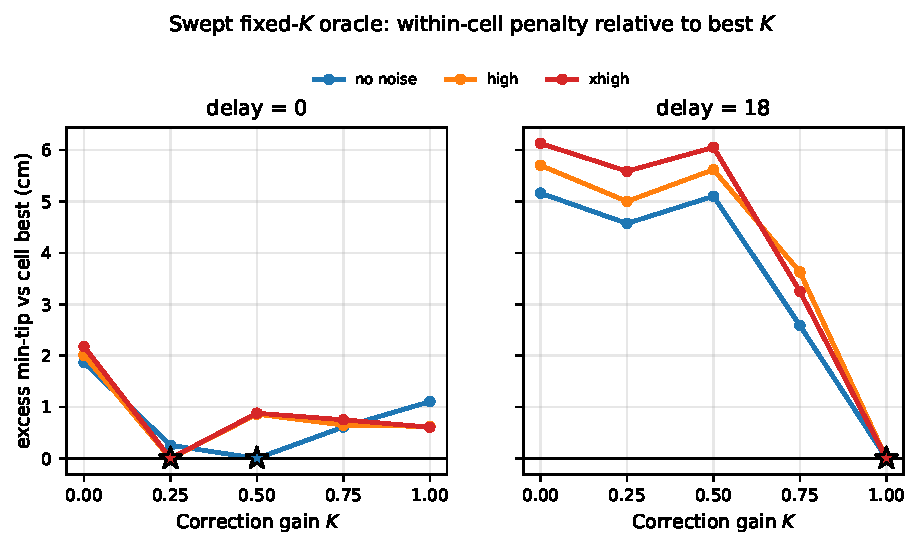
\includegraphics[width=\columnwidth]{F_r3_K_sweep.pdf}
\caption[Swept fixed-$K$ oracle: delay-dependent correction structure.]%
{\textbf{Swept fixed-$K$ closed-loop oracle is delay-dependent.}
Excess $\min$-tip error relative to the best fixed $K$ within each
noise/delay cell ($n{=}200$ episodes/cell) under the stabilized
endpoint probe across $K\!\in\!\{0,0.25,0.5,0.75,1\}$, split by
delay. Colored stars mark the per-cell best $K$ at zero penalty.
This visualization emphasizes the shape of the $K$ curve within each
cell rather than comparing absolute task difficulty between delays.
Delay-$0$ cells (left) prefer intermediate $K$, shifting toward
prediction as observation noise rises. Delay-$18$ cells (right)
collapse to $K\!=\!1$ uniformly. The closed-loop oracle is therefore
delay-dependent rather than uniformly prediction-heavy.}
\label{fig:F_r3_K_sweep}
\end{figure}

Table~\ref{tab:r3_bestK} reports the exact per-cell best $K$ and
$\min$-tip mean. The diagonal trend $K^{\star}\!=\!0.50\!\to\!0.25$
at delay-$0$ as noise rises, and the saturation at $K^{\star}\!=\!1.0$
across all delay-$18$ cells, are statistically robust under the
paired bootstrap of Sec.\,\ref{sec:results-c2} (every $K{=}0$ vs
best-$K$ contrast excludes zero at the $95\%$ percentile level).

\begin{table*}[!htbp]
\centering
\caption{Per-cell swept fixed-$K$ best $K$ and corresponding
cell-mean $\min$-tip error (m), $n{=}200$ episodes per cell,
stabilized endpoint probe, $H{=}8$ forward model, below-shoulder
target set.}
\setlength{\tabcolsep}{4pt}
\footnotesize
\begin{tabular}{@{}ll cccc cc@{}}
\toprule
noise & delay & $K{=}0.00$ & $K{=}0.25$ & $K{=}0.50$ & $K{=}0.75$ & $K{=}1.00$ & best $K$ \\
\midrule
no noise & $d{=}0$ & 0.188 & 0.172 & \textbf{0.170} & 0.176 & 0.181 & $K{=}0.50$ \\
no noise & $d{=}18$ & 0.185 & 0.180 & 0.185 & 0.160 & \textbf{0.134} & $K{=}1.00$ \\
high & $d{=}0$ & 0.188 & \textbf{0.168} & 0.177 & 0.175 & 0.174 & $K{=}0.25$ \\
high & $d{=}18$ & 0.185 & 0.178 & 0.185 & 0.165 & \textbf{0.128} & $K{=}1.00$ \\
xhigh & $d{=}0$ & 0.188 & \textbf{0.166} & 0.175 & 0.174 & 0.172 & $K{=}0.25$ \\
xhigh & $d{=}18$ & 0.185 & 0.180 & 0.185 & 0.157 & \textbf{0.124} & $K{=}1.00$ \\
\bottomrule
\end{tabular}
\label{tab:r3_bestK}
\end{table*}

\subsection{Controller-health diagnostics reclassify $K{=}0$ as an ablation (C2)}
\label{sec:results-c2}

The $K\!=\!0$ condition is valuable precisely because it reveals a
failure mode: autoregressive forward-model drift generates controller
commands that are hard to realize in muscle space. We log two
controller-health diagnostics during every closed-loop episode --- the
NNLS residual $\lVert M^{\top}a - u_{\mathrm{joint}}\rVert_{2}$ from
Eq.~(\ref{eq:nnls}), which measures how far the requested joint command
is from anything achievable by non-negative muscle activations, and
the saturation fraction of $a$ at $0.95$ --- and a paired
$95\%$ bootstrap contrast against the per-cell best fixed $K$.

Figure~\ref{fig:F_r3_k0_diagnostic}A shows the paired
$95\%$ bootstrap CI of $\min$-tip difference,
$K{=}0$ minus best $K$, per cell. The CI excludes zero in every cell;
the mean penalty is $1.9$--$2.2$\,cm at delay-$0$ cells and
$5.2$--$6.1$\,cm at delay-$18$ cells. Panel B shows the
$\mathrm{NNLS\_residual\_mean}$ heatmap: $K\!=\!0$ runs sit at
$92$--$96$ across the grid, while $K\!>\!0$ runs sit between $11$ and
$49$. The same trend holds in representative single-episode traces
(Appendix~\ref{app:artifact}): under $K\!=\!0$, the forward-model
state vector drifts by meters over the $600$-step episode, the joint
torque command requested by the task-space PD diverges, and NNLS
returns large residuals because no non-negative muscle activation
can realize that drifting command.

\begin{figure}[t]
\centering
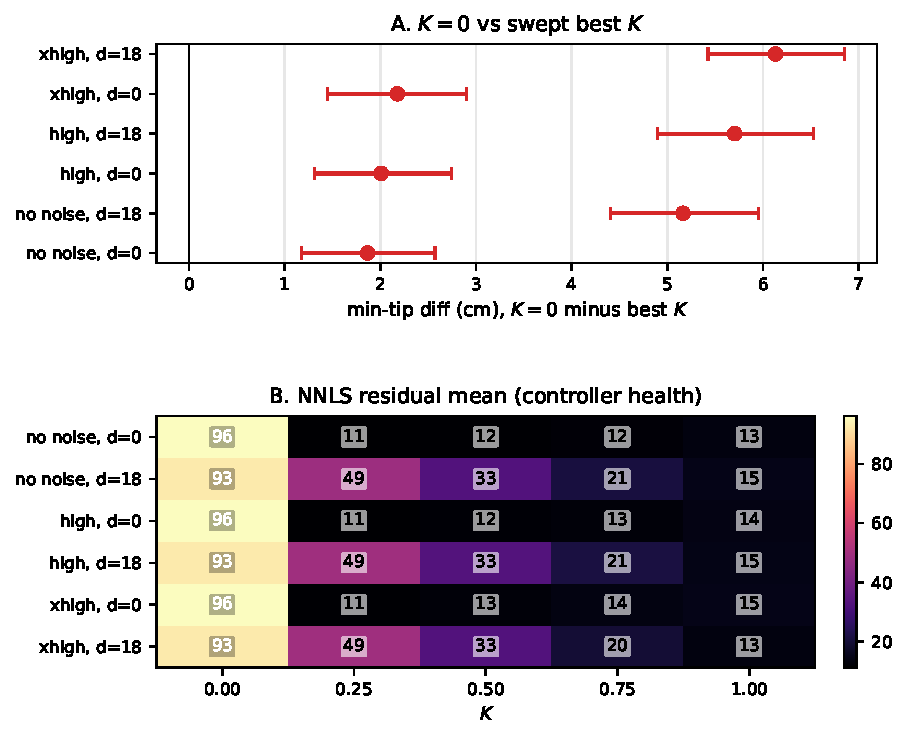
\includegraphics[width=\columnwidth]{F_r3_k0_diagnostic.pdf}
\caption[$K{=}0$ is a forward-model-only diagnostic, not the oracle.]%
{\textbf{$K{=}0$ is a forward-model-only diagnostic, not the
closed-loop oracle.} (A) Per-cell paired $\min$-tip difference
$K{=}0$ minus best fixed $K$, in cm, with $95\%$ percentile bootstrap CI
(10{,}000 resamples, paired by episode index); $K{=}0$ is systematically
worse in every cell. (B) NNLS residual mean
$\lVert M^{\top}a - u_{\mathrm{joint}}\rVert_{2}$ as a heatmap over
$K$ and cell: $K{=}0$ runs sit far above the rest of the grid,
indicating the requested joint command is unrealizable in non-negative
muscle space.}
\label{fig:F_r3_k0_diagnostic}
\end{figure}

We therefore report $K\!=\!0$ as a diagnostic ablation in all
subsequent comparisons, not as the closed-loop oracle. The
$h{=}50$ open-loop validation that selected $H{=}8$ is insufficient
to certify $K\!=\!0$ for closed-loop deployment, because the
deployment horizon is $600$ steps under a controller-induced action
distribution that the forward model never trained on; we leave
target-field clamping and controller-induced action augmentation as
future work (see Sec.\,\ref{sec:discussion}).

\subsection{Outcome-trained reliability adaptation improves delayed reaches (C3)}
\label{sec:results-c3}

We now ask whether agent-available signals --- per-episode
innovation history and per-episode $\min$-tip outcome --- can shift
the deployed correction gain toward the swept oracle.
We compare four estimators on top of the same $H{=}8$ forward
model, the same stabilized endpoint probe, and the same $200$-ep/cell
deployment:

\begin{itemize}
\item \textbf{Default reliability} ($\beta_{0,f}\!=\!0$,
$\beta_{1,f}\!=\!0.5$, all fields), an EMA-based reliability-to-gain
logistic with no training signal.
\item \textbf{Single-cell SPSA} on the no-noise, delay-$18$ cell, deployed
on that one cell only.
\item \textbf{Global SPSA $\beta$}, a single $\beta$ trained across
all six cells via outcome-only SPSA ($100$ iter, $12$ samples per
side; Sec.\,\ref{sec:method-spsa}).
\item \textbf{Feature-conditioned $\beta$}, a $30$-parameter linear
adapter that maps z-scored log innovation statistics to per-field
$\beta$ on top of the global SPSA base (Sec.\,\ref{sec:method-fc}).
\end{itemize}

For reference we also deploy a \textbf{per-cell SPSA diagnostic}
($100$ iter, $10$ samples per side, one $\beta$ per cell, deployed
on its own training cell at $n{=}200$); this is an upper bound on
what the reliability-to-gain logistic can achieve with within-cell
training and is not an agent-realistic policy.

Figure~\ref{fig:F_r3_adapt_deploy} compares the default, global,
feature-conditioned, and per-cell deployments against the swept
fixed-$K$ oracle, split by delay. At delay-$18$
cells, outcome-driven adaptation is unambiguous: global SPSA improves
on default reliability by $-1.85$\,cm in the no-noise, delay-$18$ cell,
$-2.18$\,cm at $(\mathrm{high},d{=}18)$, and $-2.46$\,cm at
$(\mathrm{xhigh},d{=}18)$, and the paired $95\%$ bootstrap CI
excludes zero in every delay-$18$ cell
(Table~\ref{tab:r3_paired_ci}). The single-cell SPSA on
the no-noise, delay-$18$ cell reduces $\min$-tip by $2.50$\,cm compared with the default on that
same cell, consistent with the global SPSA result. At delay-$0$
cells, neither global SPSA nor feature-conditioned $\beta$ improves
on default ($\Delta$ within $\pm 1$\,cm; paired CI covers zero in
every delay-$0$ cell). This split aligns directly with the
delay-dependent oracle of C1: in cells where the swept oracle
selects $K\!=\!1$, outcome-driven adaptation can find that direction;
in cells where the oracle is intermediate, the same parameterization
has little to gain over the default mid-$K$ regime.

\begin{figure}[t]
\centering
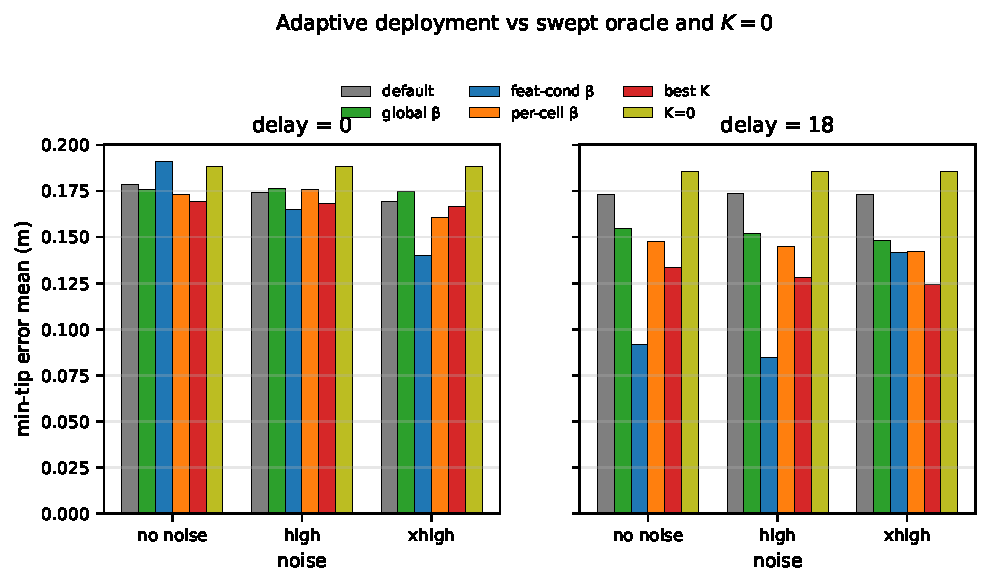
\includegraphics[width=\columnwidth]{F_r3_adapt_deploy.pdf}
\caption[Adaptive deployment vs.\ swept oracle and $K{=}0$.]%
{\textbf{Outcome-trained reliability adaptation in closed loop.}
Per-cell $\min$-tip error mean ($n{=}200$ episodes/cell) under the
stabilized endpoint probe. Bars: default reliability (gray),
global SPSA $\beta$ (green), feature-conditioned $\beta$ (blue),
per-cell SPSA diagnostic (orange), per-cell best fixed $K$ (red),
$K{=}0$ diagnostic (yellow). Adaptive estimators improve over
default at delay-$18$ cells but remain above the swept oracle by
$1.4$--$1.8$\,cm. At delay-$0$ cells, adaptive estimators sit
near default; the oracle there is intermediate $K$ rather than
observation-heavy.}
\label{fig:F_r3_adapt_deploy}
\end{figure}

The full paired-bootstrap contrast table is generated by the
reproduction pipeline in Appendix~\ref{app:repro}.

\begin{table*}[!htbp]
\centering
\caption{Key paired-bootstrap $95\%$ percentile CIs on $\min$-tip
mean differences, in meters. Each contrast is computed as the first
method named minus the second. All deploys at
$n{=}200$ episodes/cell, paired by episode index, $10{,}000$
resamples. Asterisk marks intervals that exclude zero.
The complete CSV is regenerated by the reproduction pipeline described
in Appendix~\ref{app:repro}.}
\setlength{\tabcolsep}{3pt}
\footnotesize
\begin{tabular}{@{}llrrrr@{}}
\toprule
contrast & cell & $\Delta$ & CI low & CI high & \\
\midrule
global $-$ default & no noise, $d{=}18$ & $-0.0185$ & $-0.0241$ & $-0.0131$ & * \\
 & high, $d{=}18$ & $-0.0218$ & $-0.0286$ & $-0.0154$ & * \\
 & xhigh, $d{=}18$ & $-0.0246$ & $-0.0325$ & $-0.0168$ & * \\
 & no noise, $d{=}0$ & $-0.0030$ & $-0.0083$ & $+0.0020$ & \\
 & high, $d{=}0$ & $+0.0022$ & $-0.0057$ & $+0.0095$ & \\
 & xhigh, $d{=}0$ & $+0.0054$ & $-0.0015$ & $+0.0125$ & \\
\addlinespace
feature-conditioned $-$ best $K$ & no noise, $d{=}18$ & $+0.0162$ & $+0.0097$ & $+0.0229$ & * \\
 & high, $d{=}18$ & $+0.0166$ & $+0.0092$ & $+0.0241$ & * \\
 & xhigh, $d{=}18$ & $+0.0174$ & $+0.0115$ & $+0.0235$ & * \\
\addlinespace
$K{=}0$ $-$ best $K$ & no noise, $d{=}18$ & $+0.0516$ & $+0.0441$ & $+0.0595$ & * \\
 & high, $d{=}18$ & $+0.0570$ & $+0.0489$ & $+0.0652$ & * \\
 & xhigh, $d{=}18$ & $+0.0613$ & $+0.0542$ & $+0.0685$ & * \\
 & no noise, $d{=}0$ & $+0.0187$ & $+0.0118$ & $+0.0257$ & * \\
 & high, $d{=}0$ & $+0.0201$ & $+0.0131$ & $+0.0274$ & * \\
 & xhigh, $d{=}0$ & $+0.0218$ & $+0.0144$ & $+0.0290$ & * \\
\bottomrule
\end{tabular}
\label{tab:r3_paired_ci}
\end{table*}

\subsection{The remaining gap to the swept oracle (C4)}
\label{sec:results-c4}

The feature-conditioned $\beta$ adapter does not
reach the swept fixed-$K$ oracle. Across the three delay-$18$ cells,
feature-conditioned $\beta$ minus best $K$ is $+1.6\text{--}1.7$\,cm, and the paired
$95\%$ CI excludes zero in every case
(Table~\ref{tab:r3_paired_ci}). The per-cell SPSA diagnostic, which
is the strongest within-cell reliability-to-gain learner this
parameterization allows, behaves similarly: in $5/6$ cells it is
statistically indistinguishable from feature-conditioned $\beta$,
and in $(\mathrm{xhigh},d{=}0)$ it improves on feature-conditioned $\beta$ by
$1.2$\,cm. Both estimators remain $1.4\text{--}1.8$\,cm above the
swept oracle at every delay-$18$ cell.

Figure~\ref{fig:F_r3_field_k} explains \emph{what} the adaptive rule
actually did. Under the default $(\beta_{0,f},\beta_{1,f}){=}(0,0.5)$
rule, the realized correction gain (second-half episode mean) sits
between $0.39$ and $0.92$ depending on the field. Under global SPSA, the
\texttt{qpos} gain rises to $0.88\text{--}0.98$ across cells while
\texttt{qvel} is suppressed to $0.34$. Feature-conditioned $\beta$ shifts
the same \texttt{qpos} field further toward $0.90\text{--}0.98$ on a
per-cell basis.
The adaptive rule therefore reshapes field-wise trust, not merely
scalar $K$; even so, the residual gap to the swept oracle persists,
indicating that the reliability-to-gain logistic, the cell-level
innovation features it conditions on, and the fixed-lag observer
dynamics jointly bound the achievable adaptation under
agent-available signals.

\begin{figure}[t]
\centering
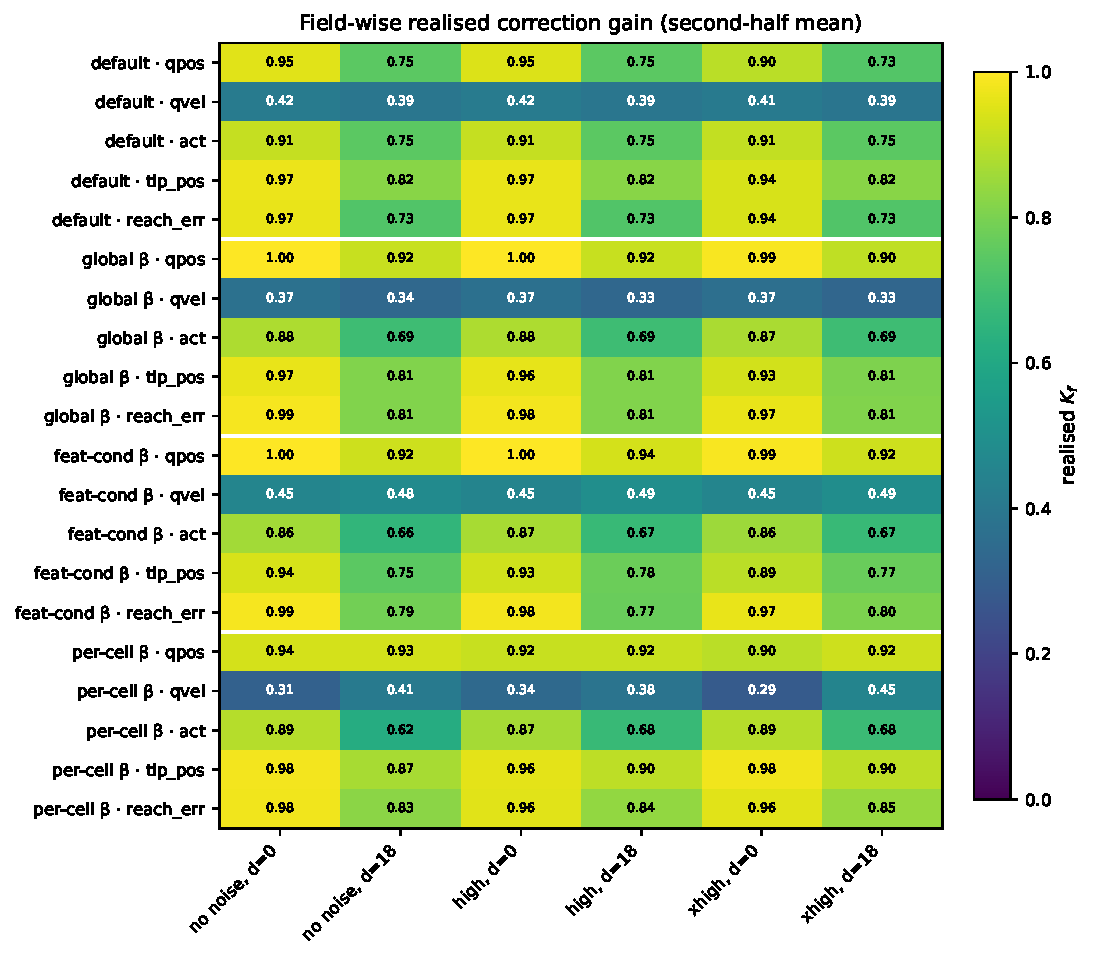
\includegraphics[width=\columnwidth]{F_r3_field_k.pdf}
\caption[Field-wise realized correction gain.]%
{\textbf{Field-wise realized correction gain (second-half episode
mean) under the four deployed estimators.} Rows: estimator $\times$
field (5 fields per estimator); columns: 6 cells. Default
reliability (top block) sits at moderate gains across fields; global
SPSA (second block) increases the \texttt{qpos} gain and suppresses
\texttt{qvel};
feature-conditioned and per-cell adapters (lower blocks) shift
field-wise trust per cell. The reliability-to-gain rule does adapt
along field-wise directions, but the residual oracle gap of C4 is
not eliminated.}
\label{fig:F_r3_field_k}
\end{figure}

The adaptive deployment summary in
Table~\ref{tab:r3_stage_c_deploy} consolidates the headline cell-mean
$\min$-tip across all five estimators plus the swept oracle and the
$K\!=\!0$ diagnostic.

\begin{table*}[!htbp]
\centering
\caption{Adaptive deployment summary, cell-mean $\min$-tip error
(m), $n{=}200$ episodes per cell. Boldface marks the smallest
$\min$-tip per row among the four adaptive estimators
(default, global $\beta$, feature-conditioned $\beta$, per-cell $\beta$).
The single-cell $\beta$ diagnostic is reported only for the no-noise,
delay-$18$ cell on which it was trained.
$K{=}0$ is shown for diagnostic comparison and is not the
closed-loop oracle (Sec.\,\ref{sec:results-c2}).}
\setlength{\tabcolsep}{3pt}
\footnotesize
\begin{tabular}{@{}ll rrrrr rr@{}}
\toprule
noise & delay & default & global & feature-cond. & per-cell & single-cell
 & $K{=}0$ & best $K$ \\
\midrule
no noise & $d{=}0$ & 0.179 & 0.176 & \textbf{0.173} & 0.173 & -- & 0.188 & 0.170 \\
no noise & $d{=}18$ & 0.173 & 0.155 & 0.150 & \textbf{0.148} & 0.148 & 0.185 & 0.134 \\
high & $d{=}0$ & \textbf{0.174} & 0.177 & 0.175 & 0.176 & -- & 0.188 & 0.168 \\
high & $d{=}18$ & 0.174 & 0.152 & \textbf{0.145} & 0.145 & -- & 0.185 & 0.128 \\
xhigh & $d{=}0$ & 0.169 & 0.175 & 0.173 & \textbf{0.161} & -- & 0.188 & 0.166 \\
xhigh & $d{=}18$ & 0.173 & 0.148 & \textbf{0.141} & 0.142 & -- & 0.185 & 0.124 \\
\bottomrule
\end{tabular}
\label{tab:r3_stage_c_deploy}
\end{table*}

% ============================================================
\section{Discussion}
\label{sec:discussion}
% ============================================================
\noindent\textbf{Delay changes the role of sensory prediction error.}
The C1 fixed-$K$ sweep separates two regimes that are hidden if
$K\!=\!0$ is treated as a usable closed-loop oracle rather than as a
forward-model-only diagnostic.
With no observation delay, the swept oracle sits at intermediate
$K\!\in\!\{0.25,0.50\}$: the predictive observer benefits from
balancing its forward-model prediction against the current sensor
reading, and increasing observation noise pushes that optimum toward
prediction, as expected from reliability-weighted prediction-error
correction. With an
$18$-step delay, the swept oracle collapses to $K\!=\!1$ in every
noise condition: the forward-model prediction at the current step is
itself stale (the observer's input is delayed by the same amount as
the observation), so observation-heavy correction wins even at the
high-noise level. We describe this only as a qualitative
reliability-weighted correction structure; the closed loop here is not
optimal control, and the observer does not propagate covariances.

\noindent\textbf{$K\!=\!0$ is a forward-model-only diagnostic.}
Under the stabilized endpoint probe, $K\!=\!0$ is systematically
worse than the per-cell best fixed $K$ in every cell, with paired
$95\%$ CIs that exclude zero; the penalty is $5.2\text{--}6.1$\,cm
at delay-$18$ cells. The NNLS controller residual at $K\!=\!0$ is
several times larger than at $K\!>\!0$, indicating that the
forward-model prediction received by the controller is not
realizable as non-negative muscle activations. This is a deployment-%
distribution gap. The open-loop $h\!=\!50$ MSE validation
selected $H{=}8$ from training data generated by random,
low-amplitude, and hold controllers; the closed-loop deployment runs
$600$ steps under a controller-induced action distribution that the forward model was
never trained on, and the autoregressive rollout drifts to
non-physical states. The implications for future work are concrete:
the target field should be invariant or clamped rather than predicted
autoregressively; training should include controller-induced action
distributions if the model is used closed-loop at low $K$; and
$h\!=\!600$ stability should be evaluated under the same action
distribution used at deployment. We retain $K\!=\!0$ on the
$K$-grid as a diagnostic to expose this failure mode, not as a
candidate oracle.

\noindent\textbf{What outcome-trained reliability adaptation can and
cannot do.} The C3 result is delay-dependent in a way that follows
directly from C1. In delay-$18$ cells, where the swept oracle is
$K\!=\!1$, outcome-driven SPSA on a single global $\beta$ moves the
realized correction toward observation-heavy correction; the
field-wise breakdown (Fig.\,\ref{fig:F_r3_field_k}) shows the
\texttt{qpos} gain rising from default $\sim\!0.72$ to $\sim\!0.89$
while \texttt{qvel} is suppressed. In delay-$0$ cells, where the swept oracle is
intermediate, the same adaptation yields no improvement over
the default mid-$K$ regime. None of these results imply that the
reliability-adaptive observer has \emph{learned the optimal Kalman
gain}: it has learned a $\beta$ that the closed-loop outcome
prefers, on a controller that is a deliberately stabilized probe,
not a biological motor planner.

\noindent\textbf{The remaining adaptation gap.}
Even feature-conditioned $\beta$, which nearly matches the per-cell
trained diagnostic in $5/6$ cells, remains $1.4\text{--}1.8$\,cm
worse than the swept fixed-$K$ oracle at every delay-$18$ cell
(Table~\ref{tab:r3_paired_ci}). Four plausible contributors:
(i)~the field-wise reliability-to-gain logistic
$K_f\!=\!\sigma(\beta_{0,f}+\beta_{1,f}\log r_f)$ is a constrained
parameterization that may not span the swept fixed-$K$ solution; (ii)~the
$10$-dimensional cell-level innovation summary used by the adapter may
not encode the cell-specific structure that determines the best fixed
$K$; (iii)~the
fixed-lag observer's recursive dynamics differ from a scalar
$K$ applied to a clean innovation, so even an oracle $\beta$ would
not necessarily reproduce the swept-$K$ outcome; (iv)~controller and
estimator are coupled, and the residual gap may reflect controller
response to imperfect state estimates rather than estimation error
itself. We do not separate these factors here; that decomposition is
left to future work.

\noindent\textbf{Scope and limitations.}
(a)~The main task is restricted to IK-reachable below-shoulder
targets. The constraint is anatomically motivated (tabletop-like
reaching) and avoids mechanically degenerate above-shoulder IK edge
solutions, but it is not a substitute for evaluation on a freely
varying set of targets.
(b)~The closed-loop controller is a stabilized probe, not a model of
biological motor planning. The NNLS routing and virtual target ramp
were introduced specifically to avoid coupled failure modes among the
controller, IK solver, and forward model; we do not claim they are how
the nervous system solves the same
problem.
(c)~All adaptive results use a single $H{=}8$ main model, a single
SPSA random seed, and a single $\beta$ parameterization. We do
not vary the forward-model architecture or supervision horizon in this
study.
(d)~The $K\!=\!0$ closed-loop instability is not necessarily a
property of any forward-model-only observer; it is a property of
this $H{=}8$ residual MLP trained on random, low-amplitude, and hold
trajectories, deployed for $600$ steps under a controller-induced
action distribution. Forward models with target-field clamping or
deployment-distribution-aware training could change the picture.
(e)~Closed-loop estimator benchmarks should carry controller-health
metrics. The artifactual $K\!=\!0$ optimum we initially observed
would not have been detectable from $\min$-tip alone; it was
detectable from NNLS residual and field-wise realized $K$.

% ============================================================
\section{Conclusion}
\label{sec:conclusion}
% ============================================================

We have presented a stabilized closed-loop benchmark for a
forward-model-based predictive state observer on a 34-muscle
musculoskeletal reaching task, together with an analysis that
separates four phenomena previously conflated by an earlier
controller diagnostic.

First, the swept fixed-$K$ closed-loop oracle is delay-dependent
(Sec.\,\ref{sec:results-c1}): at delay-$0$ cells, the best fixed $K$
is intermediate ($K\!=\!0.50$ in the no-noise cell and
$K\!=\!0.25$ at higher noise), while at delay-$18$ cells the best
fixed $K$ collapses to $K\!=\!1.0$ across all noise levels.
Second, the forward-model-only $K\!=\!0$ condition is systematically
worse than the per-cell best fixed $K$ in every cell (paired $95\%$
CIs exclude zero; mean penalty $1.9\text{--}6.1$\,cm) and shows
large NNLS controller residuals caused by long-horizon autoregressive
forward-model drift (Sec.\,\ref{sec:results-c2});
we therefore report $K\!=\!0$ as a diagnostic forward-model-only
ablation, not as a closed-loop oracle.
Third, outcome-trained reliability adaptation improves the delayed
regime: a single global $\beta$ trained via outcome-only SPSA reduces
$\min$-tip error by $1.85\text{--}2.46$\,cm versus default reliability
at every delay-$18$ cell (all paired $95\%$ CIs exclude zero), while
delay-$0$ cells remain statistically neutral
(Sec.\,\ref{sec:results-c3}); this delay-dependent benefit follows
directly from the swept-$K$ structure.
Fourth, a feature-conditioned $\beta$ adapter nearly matches a
per-cell trained reliability-to-gain diagnostic in $5/6$ cells, but
both adapters remain $1.4\text{--}1.8$\,cm worse than the swept
fixed-$K$ oracle at every delay-$18$ cell
(Sec.\,\ref{sec:results-c4}). The remaining gap indicates that the
reliability-to-gain logistic, the cell-level innovation features it
conditions on, and the fixed-lag observer dynamics jointly bound
what agent-available adaptation can deliver under this controller.

The takeaway is therefore methodological as well as substantive:
closed-loop state-estimation benchmarks need controller-health and
long-horizon diagnostics to distinguish a state-estimation finding
from artifacts caused by coupling among the controller, IK solver, and
forward model; under a
stabilized probe controller, agent-available reliability and outcome
signals can shift the deployed correction gain in the right direction
when the oracle is observation-heavy, but cannot eliminate the
remaining oracle gap with this parameterization. Future work should
train forward models on controller-induced action distributions and
test $\beta$ parameterizations richer than the field-wise logistic.

\backmatter

\bmhead{Acknowledgments}
The author thanks the MyoSuite maintainers for releasing the
musculoskeletal benchmark used in this study.

\section*{Statements and Declarations}

\noindent\textbf{Funding.} No external funding was received for this
study.

\noindent\textbf{Competing interests.} The author declares no
competing interests.

\noindent\textbf{Ethics approval.} Not applicable. This study uses
only the publicly available MyoSuite musculoskeletal simulation
environment in MuJoCo; no human, animal, or clinical data are
involved.

\noindent\textbf{Consent to participate and consent for publication.}
Not applicable (no human subjects).

\noindent\textbf{Data availability.} All main-analysis data are
generated from the MyoSuite \texttt{myoArmReachFixed-v0} environment
\cite{caggiano2022myosuite}; historical diagnostics retained in the
repository also include \texttt{myoArmReachRandom-v0}. Generation
scripts and configurations are included with the code release
(Appendix~\ref{app:repro}).

\noindent\textbf{Code availability.} The full reproduction pipeline
(dataset generation, forward-model training, closed-loop evaluation,
across-trial $\beta$ adaptation, feature-conditioned $\beta$
training, and figure generation) is released as open-source
software at
\url{https://github.com/jkoba0512/myoarm-forward-state-estimation}.
The exact software snapshot is archived at
\url{https://doi.org/10.5281/zenodo.20580300}. Frozen run identifiers required
to regenerate every numerical claim and figure are listed in
Appendix~\ref{app:repro}.

\noindent\textbf{Author contributions.} Jun Kobayashi is the sole
author and conducted all aspects of the work: conceptualization,
methodology, software, experiments, analysis, and manuscript
preparation.

% ============================================================
\begin{appendices}
\renewcommand{\theHtable}{\Alph{section}.\arabic{table}}
% ============================================================
\section{Implementation Details}
\label{app:hyperparams}

Table~\ref{tab:hyperparams} lists every hyperparameter used in the
paper. All training runs are reproducible from
\texttt{configs/} in the source repository; estimator evaluation grids
are listed verbatim in \texttt{configs/estimators/} and
\texttt{configs/closed\_loop/}.

\begin{table*}[!htbp]
\caption{Hyperparameters used across the paper.}
\label{tab:hyperparams}
\renewcommand{\arraystretch}{1.15}
\setlength{\tabcolsep}{3pt}
\scriptsize
\begin{tabular}{@{}lll@{}}
\toprule
\textbf{Component} & \textbf{Hyperparameter} & \textbf{Value} \\
\midrule
\multirow{6}{*}{Forward model $f_\theta$}
 & state dimension & 83 \\
 & action dimension & 34 \\
 & hidden layers & 2 $\times$ 256 \\
 & activation & ReLU, LayerNorm \\
 & output & residual ($\Delta x$) \\
 & parameters & 118{,}355 \\
\midrule
\multirow{6}{*}{Forward training}
 & optimizer & Adam~\cite{kingma2015adam} \\
 & learning rate & $1\,{\times}\,10^{-3}$ \\
 & weight decay & 0 \\
 & batch size & 256 \\
 & epochs & 200 (early stop patience 20) \\
 & validation split & every 5th source episode \\
\midrule
Multi-step loss
 & rollout horizon $H$ & 1, 4, 8 \\
\midrule
\multirow{4}{*}{Stabilized endpoint probe}
 & $K_p$, $K_d$ & 30, 3 \\
 & action scale $\alpha$ & 5 \\
 & ramp horizon & 300 steps \\
 & muscle routing & non-negative least squares, then clip to $[0,1]$ \\
\midrule
\multirow{3}{*}{IK solver}
 & method & damped Jacobian pseudoinverse \\
 & max iterations / tolerance & 200 / 0.01\,m \\
 & damping $\lambda^2$ & 0.1 \\
\midrule
\multirow{3}{*}{Eval grid (open-loop)}
 & noise levels & none (no noise), low, medium, high, vhigh, xhigh \\
 & delays (steps) & 0, 6, 18, 36 \\
 & $K$ values & 0.0, 0.25, 0.5, 0.75, 1.0 \\
\midrule
\multirow{2}{*}{Eval grid (closed-loop)}
 & noise levels (focused) & none (no noise), high, xhigh \\
 & delays (focused) & 0, 18 \\
\midrule
Closed-loop deploys
 & episodes per cell & 200 \\
\bottomrule
\end{tabular}
\end{table*}

\section{Forward-Model Rollout Metrics and $h{=}600$ Stability}
\label{app:fwd-rollout}

\paragraph{Open-loop rollout error.}
Table~\ref{tab:fwd_rollout} reports horizon-wise prediction error for
the main forward-model variants (single-step-supervised residual MLP on
the $77{,}292$-transition reachable-target dataset; same architecture
and training set, varied only in the rollout horizon $H$). The
$H{=}8$ main model is the one used throughout the closed-loop
results; an undertrained $H{=}8$ variant is retained for diagnostic
contrast.

\begin{table*}[!htbp]
\centering
\caption{Forward-model rollout MSE and tip prediction error on
held-out validation episodes for the reachable-target dataset (lower is better).}
\label{tab:fwd_rollout}
\setlength{\tabcolsep}{4pt}
\footnotesize
\begin{tabular}{@{}l ccc ccc@{}}
\toprule
& \multicolumn{3}{c}{MSE} & \multicolumn{3}{c}{Tip err.\ (m)} \\
\cmidrule(lr){2-4}\cmidrule(lr){5-7}
Model & $h{=}1$ & $h{=}10$ & $h{=}50$ & $h{=}1$ & $h{=}10$ & $h{=}50$ \\
\midrule
$H{=}1$ (single-step) & 0.0035 & 0.0089 & 0.0366 & 0.0040 & 0.0157 & 0.0546 \\
$H{=}4$ multi-step & 0.0037 & 0.0060 & 0.0115 & 0.0064 & 0.0206 & 0.0538 \\
$H{=}8$ multi-step (main) & 0.0038 & 0.0057 & 0.0084 & 0.0071 & 0.0162 & 0.0343 \\
undertrained $H{=}8$ & 0.0055 & 0.0082 & 0.0110 & 0.0134 & 0.0267 & 0.0517 \\
\bottomrule
\end{tabular}
\end{table*}

\paragraph{$h{=}600$ zero-action stability.}
Because the closed-loop episode is $600$ control steps long, we
additionally evaluate a zero-action autoregressive rollout from
\texttt{env.reset()} on every forward-model variant
(Table~\ref{tab:fwd_h600_stability}). The field-wise stability screen is
$|q|_{\max}\!\leq\!5$\,rad,
$|\dot q|_{\max}\!\leq\!10$\,rad/s,
tip drift on the order of the anatomical workspace ($\sim\!1$\,m),
and no NaN or Inf values.
Target drift is reported as a diagnostic field only --- all four
models drift in $p_{\mathrm{tgt}}$ because the residual-MLP predicts
the full state vector, and the target field is included in that
state; in a future iteration the target field should be clamped to
their initial value or removed from the predicted state.
In closed-loop deployments, the target channel is observed and corrected
with fixed gain $1.0$; the reported target drift therefore diagnoses only
the unconstrained open-loop rollout, not the controller-facing target
estimate.

\begin{table*}[!htbp]
\centering
\caption{Zero-action $h{=}600$ autoregressive stability per forward-%
model variant. The two $H{=}8$ variants remain bounded in
$q$/$\dot q$ and keep tip drift near the anatomical-workspace scale
(target drift treated as a diagnostic field). $H{=}1$ and $H{=}4$
diverge to non-physical states.}
\label{tab:fwd_h600_stability}
\setlength{\tabcolsep}{4pt}
\footnotesize
\begin{tabular}{@{}l rrrrr@{}}
\toprule
Model & $|q|_{\max}$ (rad) & $|\dot q|_{\max}$ (rad/s) & tip drift (m) & tgt drift (m) & status \\
\midrule
$H{=}1$ & 15.6 & 108.0 & 7.76 & 0.28 & diverges \\
$H{=}4$ & 42.4 & 217.4 & 12.6 & 10.2 & diverges \\
$H{=}8$ (main) & 1.6 & 3.9 & 1.03 & 0.54 & bounded \\
undertrained $H{=}8$ & 1.5 & 3.4 & 0.43 & 0.96 & bounded \\
\bottomrule
\end{tabular}
\end{table*}

\paragraph{Closed-loop $K{=}0$ instability.}
Under $K{=}0$ the same $H{=}8$ main model is driven by a controller-%
induced action sequence (rather than zero action) and the rollout
diverges much more aggressively (e.g.\ $|q|_{\max}{=}11.8$\,rad,
$|\dot q|_{\max}{=}29.6$\,rad/s, tip drift $8.76$\,m at the same
$600$-step horizon). The gap between the zero-action and the
closed-loop $K{=}0$ rollouts is the deployment-distribution gap
discussed in Sec.\,\ref{sec:results-c2}; it motivates including
controller-induced action distributions in future forward-model
training.

\clearpage
\section{Below-Shoulder Target Set and Historical Controller Diagnostic}
\label{app:artifact}

The main target set is generated by uniformly sampling the
environment's task-space reach bounding box, applying a damped-Jacobian
IK acceptance test (tolerance $1$\,cm), and rejecting candidates above
the neutral shoulder height ($z\!=\!1.393$\,m). This shoulder-height
criterion is anatomical, not a post-hoc performance filter: it removes
mechanically degenerate above-shoulder reaches that the IK solver can
satisfy only by pinning several shoulder/scapula joints to range
limits. The acceptance rate is $55.9\%$ for $n{=}200$ accepted targets;
after the shoulder-height filter, the IK tolerance test rejects $0\%$
of candidates.

The change to the stabilized endpoint controller was motivated by an
earlier diagnostic that used a one-shot IK pre-solve, a joint-space PD
controller, a ReLU-then-moment-arm muscle map, and an unrestricted
target set. That diagnostic produced a misleading apparent optimum at
$K\!=\!0$: high-reaching targets pinned joints, the muscle map could not
realize the resulting joint command, and long-horizon forward-model
autoregression drifted to non-physical states. The stabilized endpoint
probe (Sec.\,\ref{sec:method-controller}) and the below-shoulder target
set remove these failure modes; the historical diagnostic is not used
as a main result.

\section{Software, Hardware, and Reproducibility}
\label{app:repro}

\paragraph{Software stack.} Python 3.11, PyTorch configured for CPU execution, MuJoCo
3.x, Gymnasium~0.29, MyoSuite~2.12.2, NumPy, SciPy, pandas, and
matplotlib. Project-level dependencies are pinned in
\texttt{pyproject.toml}.

\paragraph{Hardware.} All experiments were run on a single CPU
workstation (no GPU required). Forward-model training takes
$\sim\!30$\,min per model. A small fixed-$K$ diagnostic sweep of
$300$ episodes ($5$ values of $K$ $\times\,6$ cells $\times\,10$ episodes)
takes $\sim\!10$\,min; the main $200$-episode-per-cell deployment
tables take proportionally longer. Per-cell SPSA training ($100$ iterations,
$S\!=\!10$, $20$ episodes per iteration) takes $\sim\!1$\,hour per
cell when run alone; the $200$-iteration feature-conditioned
$\beta$ training (Sec.\,\ref{sec:method-feature-cond}) takes
$\sim\!3.5$\,hours.

\paragraph{Main reproduction path.}
The repository contains executable configuration files for each training,
evaluation, and plotting step. The main numerical tables and figures are
regenerated from the
fixed-gain closed-loop sweep config, the adaptive-deployment configs, the
paired-bootstrap wrapper, and the paper-figure builder listed in the released
source tree. The forward-model and SPSA training commands are listed in
\texttt{configs/models/} and \texttt{configs/train/}; each run writes
its config and Git commit hash to \texttt{runs/}.

\paragraph{Historical reproduction.}
Earlier joint-PD diagnostics are retained in the repository for auditability but
are excluded from the main analysis because they used the unrestricted target
set and controller pipeline described in Appendix~\ref{app:artifact}. They
should not be used to reproduce the stabilized-controller results.

\paragraph{Repository layout.}
\begin{footnotesize}
\begin{verbatim}
src/myoarm_fse/
 envs/ MyoSuite wrappers, observation pipelines
 models/ ForwardMLP, training loops
 estimators/ FixedGainKalman, ReliabilityAdaptive, Learned
 controllers/ JointSpacePD, EndpointError
 controllers/ BC kept for historical runs
 evaluation/ closed_loop.py (single episode rollout)
scripts/ training, evaluation, and plotting entries
configs/
 models/ forward-model training configs
 closed_loop/ closed-loop eval configs
 train/ SPSA and per-cell SPSA configs
 train/ feature-conditioned beta configs
runs/ local outputs; large artifacts not versioned
figures/ committed PDF/PNG of paper figures
paper/ LaTeX source + bibliography
\end{verbatim}
\end{footnotesize}

\paragraph{Tests.}
Unit tests cover the per-step observer math, fixed-lag delay
handling, and the deterministic build of every estimator. A
MyoSuite-marked smoke suite verifies that one closed-loop episode
runs end-to-end with each controller-estimator combination. The
reproduction checklist uses:
\begin{footnotesize}
\begin{verbatim}
uv run pytest # default fast tests
uv run pytest -m myosuite # closed-loop integration smoke
\end{verbatim}
\end{footnotesize}

\paragraph{Run artifacts.}
The repository includes configs that, when run, write reproducible
output directories under \texttt{runs/}. Each closed-loop or
training run records its resolved config and a Git commit hash in
\texttt{config.json}, so re-running with the same seed and commit
reproduces the reported seeded outputs. Frozen run identifiers are
embedded in the configs and wrapper scripts listed above, and are kept
there rather than repeated in the manuscript text.

\end{appendices}

\bibliography{refs}

\end{document}
